\section{Busqueda lineal}
%\subtitle{Ejercicio 1}

El primer algoritmo analizado fue el algoritmo básico de busqueda, el primero en el que pensaría cualquiera cuando se le plantea el problema, que no es mas que recorrer el vector hasta encontrar el elemento buscado. De esta descripción se aprecia claramente que en su peor caso es lineal, ya que habria que recorrer todo el vector, si el elemento buscado aparece en la ultima posición.

\subsection{Analisis de eficiencia teorico}


El desarrollo matemático de el analisis de la eficiencia teoríca del codigo del algoritmo que se muestra arriba es el siguiente:

% formula aqui

Tras hacer pruebas con distintos tamaños de entradas se ha obtenido la siguiente grafica de tiempos, en la cual se enfrenta el tamaño del vector en el que se ha buscado aplicando el algoritmo (eje x) y el tiempo que ha tardado en completarse el algoritmo para cada tamaño.

\begin{figure}[h]
  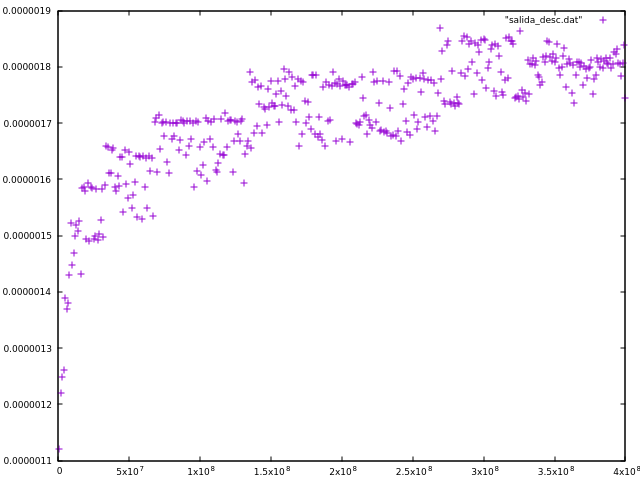
\includegraphics[width=0.5\textwidth]{./Imagenes/binaria_data.png}
  \caption{Datos de la salida del algoritmo de busqueda lineal}
\end{figure}
